\documentclass{beamer}
\usepackage{amsmath}
\usepackage{amssymb}
\usepackage{physics}
\usepackage{amsthm}
\usepackage{graphicx}
\usepackage{caption}
\usepackage{subcaption}
\graphicspath{ {./figures/} }
\title{Spektrální metoda a Kmitání membrán}
\author{Dominika Hájková, Matyáš Fuksa, Ondřej Kureš}
\institute{Stormtrooperz}
\date{2021}

\begin{document}

\frame{\titlepage}

\begin{frame}
\frametitle{Spektrální metoda aneb trám jinak}
Zatím jen rozvržení.
\end{frame}
\begin{frame}
\frametitle{Kmitání membrán}
Zatím jen rozvržení.
\end{frame}


\begin{frame}
\begin{center}
\begin{huge}
Děkujeme za pozornost
\end{huge}
  \centering
  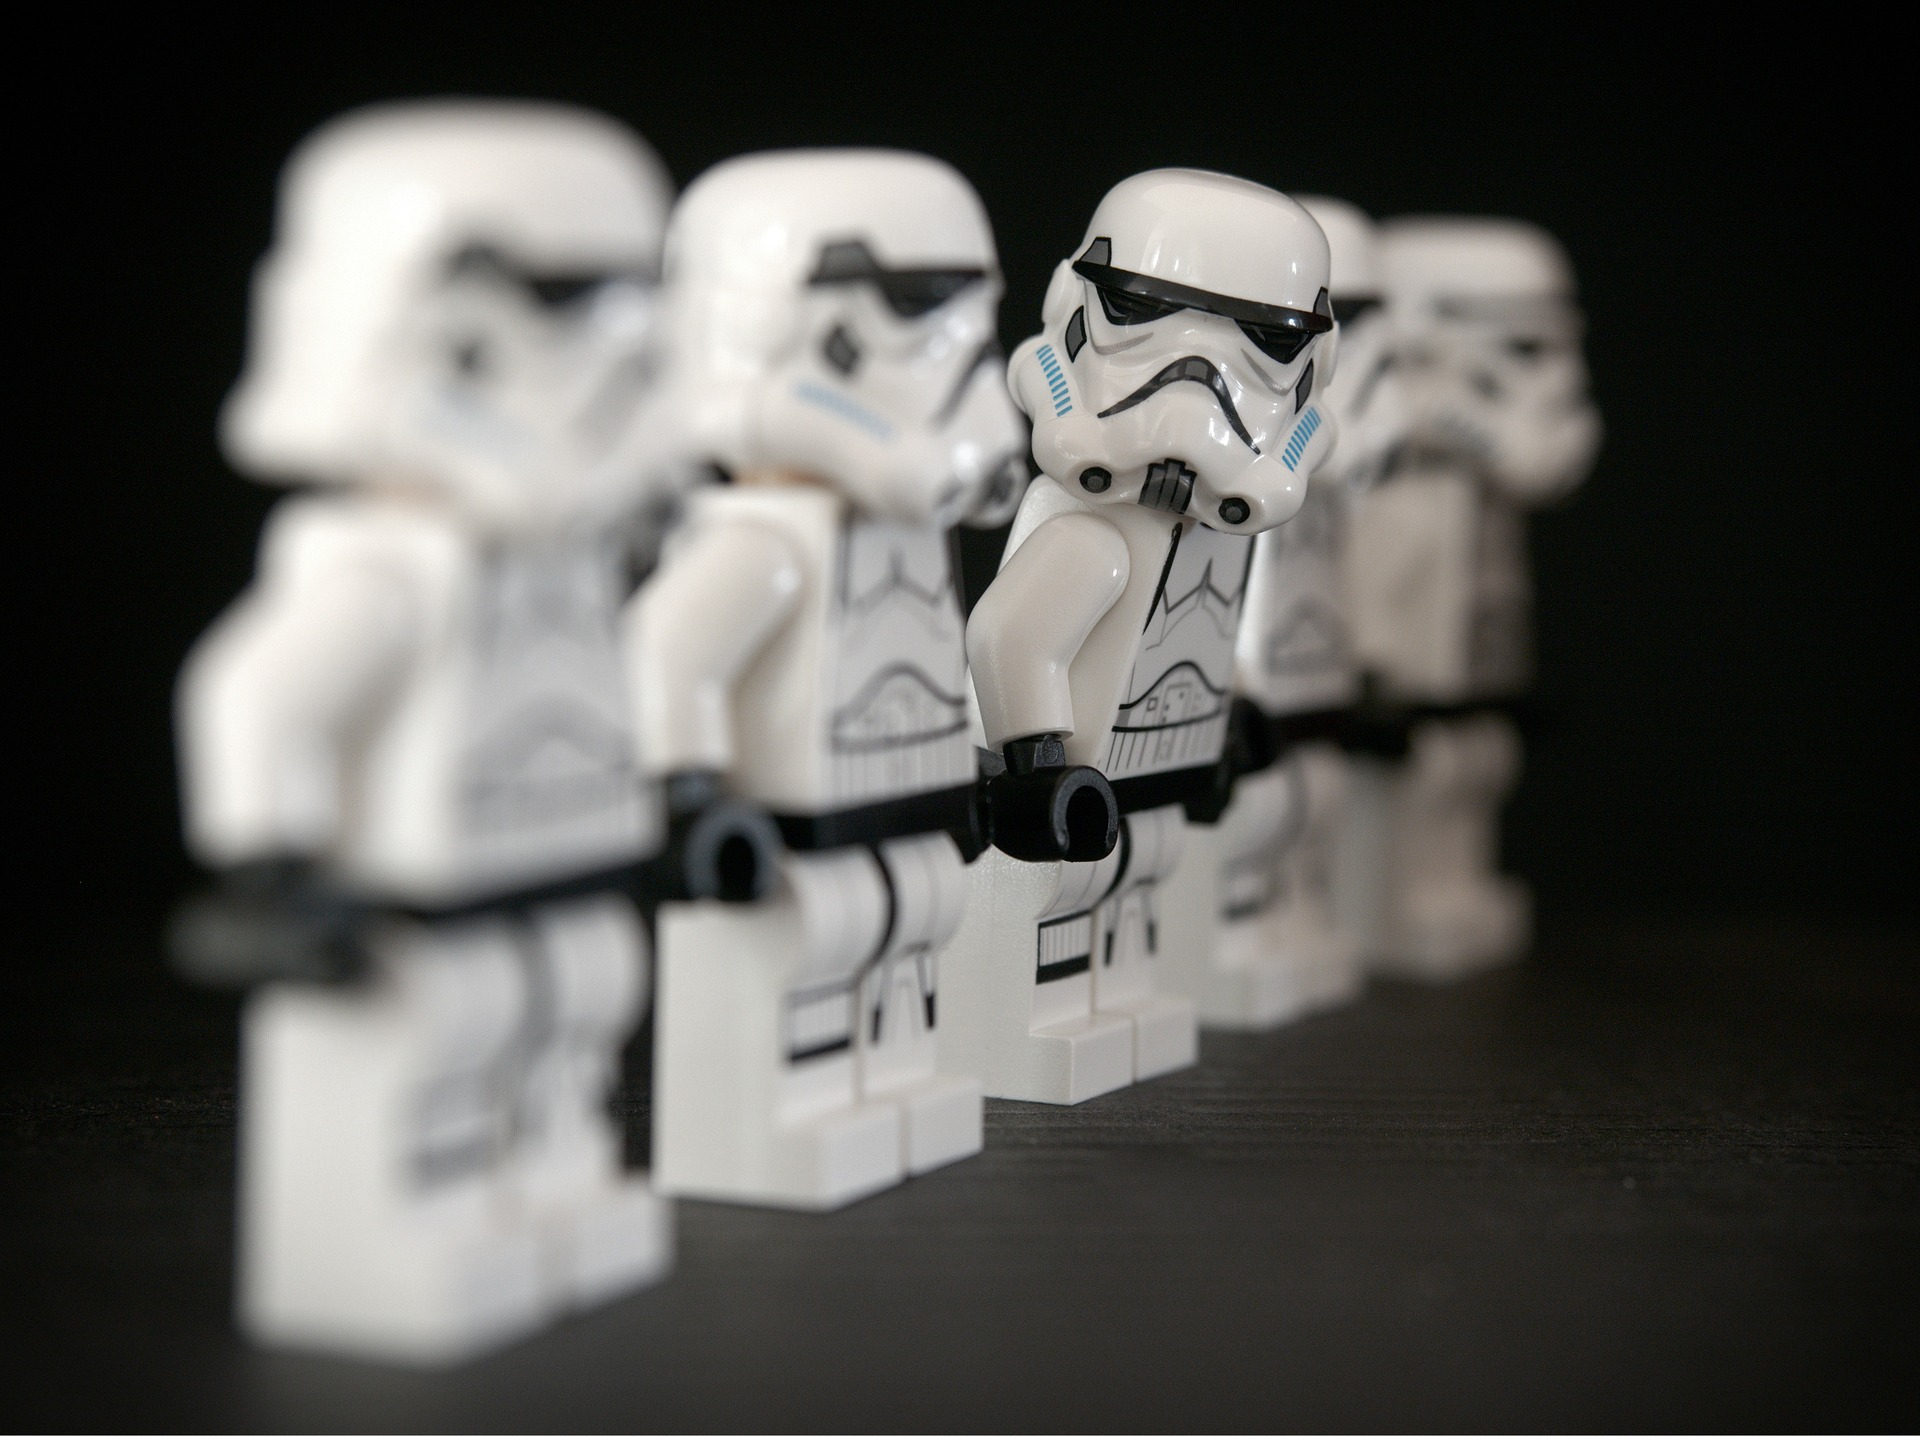
\includegraphics[width=.8\linewidth]{stormtroop.jpg}
\end{center}

\end{frame}
\end{document}